\documentclass[11pt,a4paper]{article}
\usepackage[T1]{fontenc}
\usepackage{amsmath,amsthm}
\usepackage{newtxtext,newtxmath}
\usepackage[margin=24mm]{geometry}
\usepackage{microtype,booktabs,tabularx,array}
\usepackage{xcolor,graphicx,tikz}
\usetikzlibrary{arrows.meta,positioning,fit,backgrounds}
\usepackage{listings}
\usepackage[section]{placeins}
\usepackage[colorlinks=true,allcolors=blue!45!black]{hyperref}
\usepackage{enumitem}
\hypersetup{pdftitle={Event-Driven Hierarchical Rule Composition and Saturation},pdfsubject={Saturated rule compositions and fractal-composition feedback},pdfkeywords={egraph, equality saturation, saturated rule composition, dissipative, infi}}
\setlist{nosep,leftmargin=*}
\setlength{\parskip}{4pt}
\setlength{\parindent}{1em}
\setlength{\emergencystretch}{2em}
\newtheorem{definition}{Definition}
\newtheorem{proposition}{Proposition}
\newtheorem{remark}{Remark}
\newcommand{\Cl}{\operatorname{Cl}}
\newcommand{\CS}{\mathsf{CS}}
\newcommand{\Seq}{\mathsf{Seq}}
\newcommand{\Par}{\mathsf{Par}}
\newcommand{\Ready}{\mathsf{Ready}}
\newcommand{\Unknown}{\mathsf{Unknown}}
\newcommand{\code}[1]{\texttt{#1}}
\lstset{basicstyle=\ttfamily\footnotesize,columns=fullflexible,keepspaces=true,
 breaklines=true,frame=single,rulecolor=\color{black!20},backgroundcolor=\color{black!2},
 xleftmargin=3pt,xrightmargin=3pt,aboveskip=7pt,belowskip=7pt}
\tikzset{box/.style={draw=black!50,rounded corners,align=center,fill=black!2,
 minimum height=9mm,text width=37mm,font=\small,inner sep=4pt},
 arr/.style={-{Latex[length=2mm]},draw=black!65},
 proposed/.style={arr,dashed},coarse/.style={box,draw=violet!70!black,very thick,fill=white},
 smooth/.style={box,draw=teal!75!black,dashed,thick,fill=white}}
% Separate notations: dashed enclosures = e-classes; solid small boxes = e-nodes.
% Diagram arrows are explicitly labelled when they denote execution or catalog
% references rather than child slots. No colour memorisation is required.
\tikzset{en/.style={draw,rounded corners=1pt,fill=white,inner sep=3pt,font=\small},
 ec/.style={draw,dashed,rounded corners,inner sep=5pt},
 note/.style={align=center,font=\small},
 rec/.style={draw,align=center,text width=43mm,inner sep=5pt,font=\small}}
\newcommand{\TeachingReplay}{%
\begin{figure}[!htbp]\centering
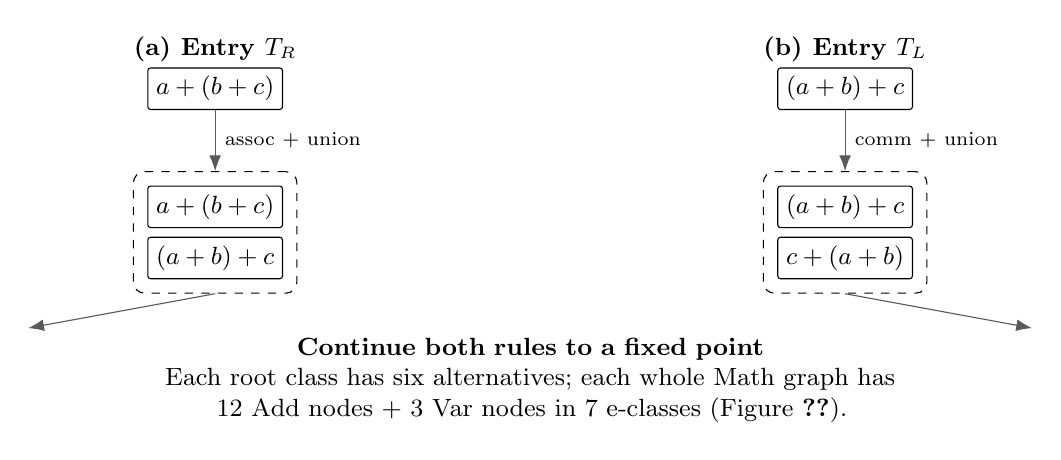
\begin{tikzpicture}
\node[note] at (0,0.5) {\textbf{(a) Entry $T_R$}};
\node[note] at (8,0.5) {\textbf{(b) Entry $T_L$}};
\node[en] (r) at (0,0) {$a+(b+c)$};
\node[en] (l) at (8,0) {$(a+b)+c$};
\node[en] (r1) at (0,-1.5) {$a+(b+c)$};
\node[en] (r2) at (0,-2.15) {$(a+b)+c$};
\node[en] (l1) at (8,-1.5) {$(a+b)+c$};
\node[en] (l2) at (8,-2.15) {$c+(a+b)$};
\node[ec,fit=(r1)(r2)] (rc) {};
\node[ec,fit=(l1)(l2)] (lc) {};
\draw[arr] (r)--node[right,font=\scriptsize]{assoc + union}(rc);
\draw[arr] (l)--node[right,font=\scriptsize]{comm + union}(lc);
\node[note,text width=125mm] (end) at (4,-3.7)
 {\textbf{Continue both rules to a fixed point}\\
 Each root class has six alternatives; each whole Math graph has\\
 12 Add nodes + 3 Var nodes in 7 e-classes (Figure~\ref{fig:body}).};
\draw[arr] (rc.south)--(end.north west);
\draw[arr] (lc.south)--(end.north east);
\end{tikzpicture}
\caption{Two familiar expressions, two local executions. Dashed enclosures show
one root e-class with retained alternatives. Expressions abbreviate e-node graphs;
child classes are expanded in Figure~\ref{fig:body}. Labelled arrows denote
selected rewrite steps, not deletion or replacement of the original expression.
The intermediate panels explain individual applications; the automated ripen test
checks the final fixed points rather than prescribing these first applications.}
\label{fig:replay}
\end{figure}}

\newcommand{\TeachingCatalog}{%
\begin{figure}[!htbp]\centering
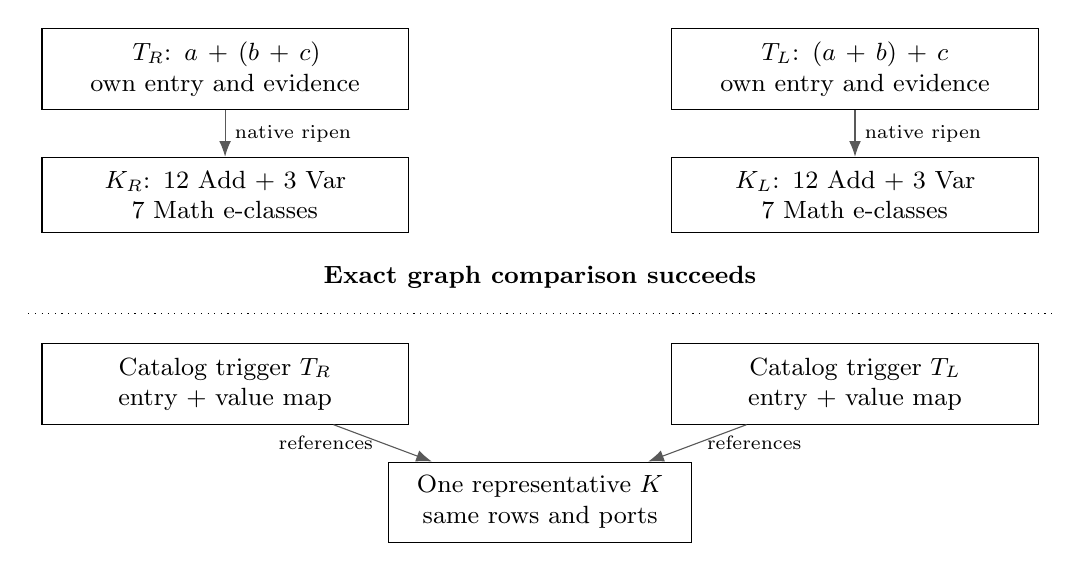
\begin{tikzpicture}
\node[rec] (r) at (0,0) {$T_R$: $a+(b+c)$\\own entry and evidence};
\node[rec] (l) at (8,0) {$T_L$: $(a+b)+c$\\own entry and evidence};
\node[rec] (kr) at (0,-1.6) {$K_R$: 12 Add + 3 Var\\7 Math e-classes};
\node[rec] (kl) at (8,-1.6) {$K_L$: 12 Add + 3 Var\\7 Math e-classes};
\draw[arr] (r)--node[right,font=\scriptsize]{native ripen}(kr);
\draw[arr] (l)--node[right,font=\scriptsize]{native ripen}(kl);
\node[note] at (4,-2.65) {\textbf{Exact graph comparison succeeds}};
\node[rec] (tr) at (0,-4) {Catalog trigger $T_R$\\entry + value map};
\node[rec] (tl) at (8,-4) {Catalog trigger $T_L$\\entry + value map};
\node[rec,text width=35mm] (k) at (4,-5.5) {One representative $K$\\same rows and ports};
\draw[arr] (tr)--node[left,font=\scriptsize]{references}(k);
\draw[arr] (tl)--node[right,font=\scriptsize]{references}(k);
\draw[dotted] (-2.5,-3.1)--(10.5,-3.1);
\end{tikzpicture}
\caption{Before comparison: two completed replay exports. After comparison:
two catalog trigger records reference one representative body. Solid rectangles
are records, not e-classes. Equal counts alone do not justify either reference:
the checker requires a complete typed bijection preserving roots, rows, and
visibility. Per-run exports and the live tier0 graph are not deleted.}
\label{fig:catalog}
\end{figure}}

\newcommand{\TeachingBody}{%
\begin{figure}[!htbp]\centering
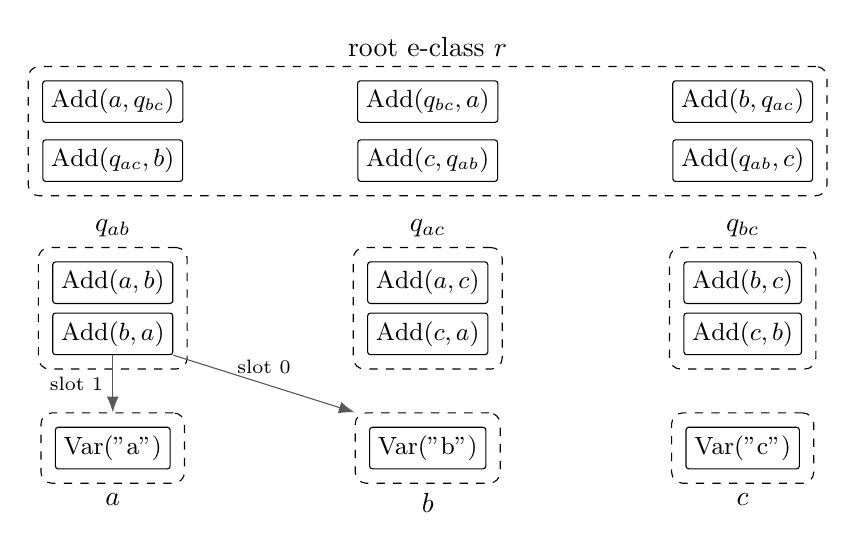
\begin{tikzpicture}
\node[en] (r0) at (0,0) {$\mathrm{Add}(a,q_{bc})$};
\node[en] (r1) at (4,0) {$\mathrm{Add}(q_{bc},a)$};
\node[en] (r2) at (8,0) {$\mathrm{Add}(b,q_{ac})$};
\node[en] (r3) at (0,-0.75) {$\mathrm{Add}(q_{ac},b)$};
\node[en] (r4) at (4,-0.75) {$\mathrm{Add}(c,q_{ab})$};
\node[en] (r5) at (8,-0.75) {$\mathrm{Add}(q_{ab},c)$};
\node[ec,fit=(r0)(r1)(r2)(r3)(r4)(r5),label=above:{root e-class $r$}] {};
\node[en] (ab0) at (0,-2.3) {$\mathrm{Add}(a,b)$};
\node[en] (ab1) at (0,-2.95) {$\mathrm{Add}(b,a)$};
\node[ec,fit=(ab0)(ab1),label=above:{$q_{ab}$}] (ab) {};
\node[en] (ac0) at (4,-2.3) {$\mathrm{Add}(a,c)$};
\node[en] (ac1) at (4,-2.95) {$\mathrm{Add}(c,a)$};
\node[ec,fit=(ac0)(ac1),label=above:{$q_{ac}$}] {};
\node[en] (bc0) at (8,-2.3) {$\mathrm{Add}(b,c)$};
\node[en] (bc1) at (8,-2.95) {$\mathrm{Add}(c,b)$};
\node[ec,fit=(bc0)(bc1),label=above:{$q_{bc}$}] {};
\node[en] (a0) at (0,-4.4) {Var("a")};
\node[en] (b0) at (4,-4.4) {Var("b")};
\node[en] (c0) at (8,-4.4) {Var("c")};
\node[ec,fit=(a0),label=below:{$a$}] (a) {};
\node[ec,fit=(b0),label=below:{$b$}] (b) {};
\node[ec,fit=(c0),label=below:{$c$}] {};
\draw[arr] (ab1.south)--node[left,font=\scriptsize]{slot 1}(a.north);
\draw[arr] (ab1.south east)--node[above,font=\scriptsize]{slot 0}(b.north west);
\end{tikzpicture}
\caption{Count and read the entire saturated Math body. Each solid box is one
e-node; each dashed enclosure is one e-class. The ordered labels specify all
child-class references. Two arrows expand the slots of Add$(b,a)$ as a reading
example; the other references remain explicit in the labels. There are six root
Add nodes, six pair Add nodes, and three Var nodes. Primitive String values are
omitted. Only association and commutation are enabled.}
\label{fig:body}
\end{figure}}

\newcommand{\TeachingBoundary}{%
\begin{figure}[!htbp]\centering
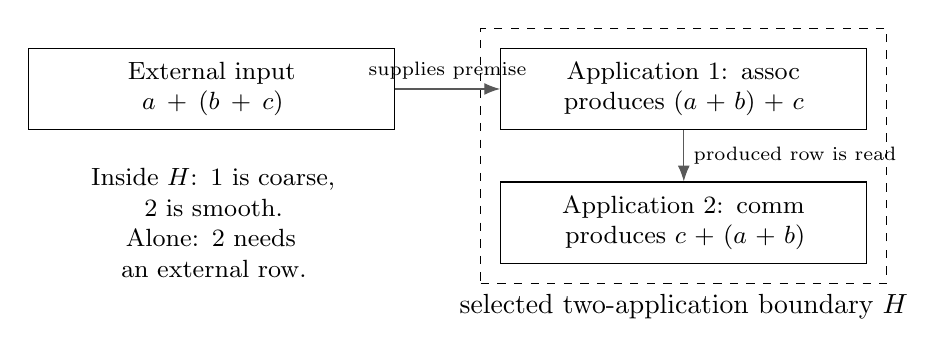
\begin{tikzpicture}
\node[rec] (i) at (0,0) {External input\\$a+(b+c)$};
\node[rec] (a) at (6,0) {Application 1: assoc\\produces $(a+b)+c$};
\node[rec] (b) at (6,-1.7) {Application 2: comm\\produces $c+(a+b)$};
\draw[arr] (i)--node[above,font=\scriptsize]{supplies premise}(a);
\draw[arr] (a)--node[right,font=\scriptsize]{produced row is read}(b);
\node[draw,dashed,fit=(a)(b),inner sep=7pt,label=below:{selected two-application boundary $H$}] {};
\node[note,text width=42mm] at (0,-1.7) {Inside $H$: 1 is coarse,\\2 is smooth.\\Alone: 2 needs an external row.};
\end{tikzpicture}
\caption{The boundary changes the role, not the rule. Rectangles represent
application or input records; the dashed enclosure is the selected history
fragment, not an e-class. The dependency arrow identifies a producer-to-consumer
row witness. Moving application 1 outside the boundary makes that dependency
external for application 2.}
\label{fig:boundary}
\end{figure}}

\title{Event-Driven Rule Composition and Local Saturation\\[5pt]
\large From Recorded Dependencies to Comparable Saturated Bodies}
\author{}
\date{Technical report \quad 21 September 2026\\
\small Teaching revision v0.3}
\begin{document}
\maketitle
\begin{abstract}
Different rule applications can reach the same local e-graph through different
entries and histories. We study how to record that common result without losing
the conditions under which each computation was valid. Our finite pipeline extracts
witnessed interfaces, constructs bounded composition candidates, validates them in
isolated native egglog executions, runs local saturation, and compares the exported
bodies. Coarse and smooth rule compositions describe dependencies relative to a
chosen boundary; CSCS and CCSS are candidate construction strategies. Cataloguing
identical bodies retains separate entry and evidence records. A small native
regression demonstrates this distinction with two entries and one representative
body. Historical experiments demonstrate recursive descriptor construction, but do
not measure native runtime compression or acceleration. Parameterized recurrence
summaries are discussed separately as a possible extension requiring additional
proof obligations.
\end{abstract}

\section{Start with two computations}
An e-graph stores alternative expressions in equivalence classes. Egglog combines
this representation with relational reasoning~\cite{egglog}. Our question concerns
a different object: can we recognize when two \emph{local computations} have the
same result, while keeping their entry conditions separate?

Use a small fragment of \path{math.egg}: symbolic variables, addition, the
associativity rewrite $a+(b+c)\Rightarrow(a+b)+c$, and commutation
$a+b\Rightarrow b+a$. The variables denote formal algebraic terms, so no
floating-point reassociation is involved. Entry $T_R$ declares
$\mathit{root}=a+(b+c)$; entry $T_L$ declares $\mathit{root}=(a+b)+c$.
These are separate local executions.
\begin{lstlisting}
(datatype Math (Var String) (Add Math Math))
(rewrite (Add a (Add b c)) (Add (Add a b) c))
(rewrite (Add a b) (Add b a))
; Right-associated entry; change only this entry for the second run.
(let root (Add (Var "a") (Add (Var "b") (Var "c"))))
\end{lstlisting}
The rewrites introduce alternatives and union their results; they retain the
original expressions. Figure~\ref{fig:replay} follows a selected first application
from each entry. Continuing both rules reaches the same body shown in
Figure~\ref{fig:body}: 12 Add nodes and three Var nodes in seven Math e-classes.
\TeachingReplay
\TeachingBody

To compare the bodies, preserve the named root, map the three variable classes
by their literal names, and map each pair class by its children. Every retained
Add row then corresponds. The initial entries still differ.
Figure~\ref{fig:catalog} records this distinction: retain two entry records and
associate them with one representative body. Both native replays have already
occurred when comparison is made.
\TeachingCatalog

This example establishes an equality of results. It says nothing about avoiding
either replay, reducing live matcher work, or deleting facts from the source
e-graph. Those require an execution mechanism and measurements beyond this
catalog. The rest of the report follows one path: represent a candidate, construct
it from evidence, replay it, saturate it, and compare the result.

\section{Represent the boundary before composing}
\subsection{Three objects with different jobs}
A \emph{candidate} is a selected set of recorded applications and a proposed
interface. A \emph{body} is the typed graph exported after an isolated run. A
\emph{saturated rule composition} associates a successfully validated candidate
and its entry contract with a saturated body:
\[
 U=(I,J,M,\Pi,K).
\]
Here $I$ is the entry and binding map, $J$ the staged external obligations, $M$
the source members, $\Pi$ the validation evidence, and $K$ the body. Body comparison
operates on $K$; activation depends on $I$ and $J$.

The repository currently distributes this object over files. The Rust type named
\code{SaturatedRuleComposition} stores the body, including typed values, rows,
visibility, scope, and fixed ports. The ripen report and catalog trigger records
hold entry and provenance information. Thus the type alone is not the complete
$U$ above. No new runtime representation is claimed by this notation.

\subsection{Applications, facts, and dependency witnesses}
A logical rule match, a surviving action, and an inserted row are different
observations. The importer uses recorded producer and equality evidence when it
forms dependencies. Sharing a value is a useful reason to inspect two applications;
it does not by itself establish that one consumed the other's committed result.
The supported imported history is subject to the trace and source-coverage checks.

A port map says whether an input comes from an earlier member, a carried input,
or an external obligation. It must preserve types and aliases. For example,
commutation of $v+c$ after associativity of $a+(b+c)$ uses $v=[a+b]$ and carries
$c$. The input map is a structural connection, not a numeric binding offset.

\subsection{Coarse and smooth are relative roles}
A \emph{coarse rule composition} needs an external obligation not yet supplied
inside the selected boundary. A \emph{smooth rule composition} has its relevant
dependencies explained by that interface and earlier internal evidence. The same
application may receive a different classification when its suppliers are included
in a larger boundary. This classification uses the selected witness; it does not
search all possible proofs for a minimal boundary.
\TeachingBoundary

In Figure~\ref{fig:boundary}, the associativity step needs the input row. Its
commutation consumer can use the produced row inside the two-member unit. If the
consumer is considered alone, that same row becomes an external obligation.
Neither classification implies termination, repeated structure, or profitable
sharing. Those are separate questions.

\section{Construct candidates from recorded history}
The candidate builder operates on application descriptors. It does not execute a
new rule. A Use, an occurrence of an installed combination template, is one
candidate source. The default composition path also builds CS units from observed
coarse and smooth layers. Bounded ancestor cones are an alternative experimental
admission strategy.

\subsection{Dependency composition: CSCS}
When one unit consumes another's output and the dependency direction is consistent,
the builder may propose a sequential pair. The stored port links explain which
inputs are internal and which still require external supply. Transitive checks
include paths through events outside the pair. Mutually dependent whole units
cannot simply be concatenated; the pair is skipped or needs finer decomposition.

\subsection{Conditional regrouping: CCSS}
The second strategy inspects disjoint units with intersecting coarse ports. It
requires supported positive constructor/relation/equality operations and checks
that no coarse member transitively depends on a smooth member. Under a complete
witness and appropriately available external inputs, those conditions permit a
C-before-S topological grouping. They do not move a late external input earlier.

The implementation records this admission condition and validates the original
staged sequence. It does not execute a reordered CCSS schedule. We therefore call
CCSS a \emph{conditional regrouping candidate}, rather than a parallel operator or
a separate saturation algorithm.

\subsection{Budgets and event subscriptions}
Resource changes awaken subscribed descriptors for further bounded pairing.
Union aliases, table changes, and scope invalidation determine which recorded
instances need attention. This is an implementation optimization for discovery,
not a proof of a live whole-graph embedding. Each proposed composition still needs
native validation.

The store limits CS versions to 256, members per composite to 16, proposals per
kind to 64, indexed alternatives per token to eight, and partners considered per
awakened unit to 32. Dependency traversal is separately bounded. A missed pair
means the search was incomplete, not that no useful composition exists. These
limits bound selected bookkeeping operations; they do not bound the cost of one
native rule call or the complete pipeline.

\section{Validate, then saturate an isolated entry}
\subsection{Reconstruct the obligations}
Entry extraction translates recorded bindings into executable terms. Unsupported
external e-class structure becomes an opaque \code{RipenInput} parameter.
Repeated parameter indices preserve identity; distinct indices are initially
unmerged. These terms are boundary markers, not wildcards matching arbitrary
external structure.

The extractor checks original premises and recorded output aliases around ground
actions. For member-based candidates, supported external rows are injected at
recorded stages. The emitted setup includes those stages before ordinary ripen
sweeps begin. The Use path has stricter admission and rejects late producers and
unsupported staging. Neither path reconstructs arbitrary outside state.

A missing guard must be supplied as an obligation. Knowing the denominator $b$
in a division rule does not derive \code{is-not-zero}$(b)$. Likewise, pre-creating
a term that should have been produced internally can change the entry contract;
the extractor rejects unsupported cases rather than using that shortcut.

\subsection{Run the native engine}
Ripen creates an isolated native engine, executes the prepared setup, and sweeps
the declared rulesets. A complete sweep without updates yields \code{Saturated}.
If the round budget ends while updates continue, the result is \code{Suspended}.
\code{Pending} means no job has run; \code{Rejected} means extraction or validation
failed. Saturation and export are separate: a run may reach a fixed point while
its state lies outside the supported export contract.

The fixed point belongs to the declared entry and schedule. Substituting concrete
terms for opaque parameters can expose additional matches. Thus a local result
cannot certify every embedding into tier0.

\subsection{What promotion feeds back}
After an eligible composition passes validation and exports a body, promotion
creates a new descriptor with inherited source members and increased depth. A
later composition flattens those member references and prepares another replay.
It does not start by merging the already saturated bodies, reuse native join
state, or install an executable macro. The recursion is in candidate descriptors.

\section{Compare bodies, preserve entries}
The body records typed values, constructor and supported table rows, canonical
equality-class references, named ports, visibility, and the exported environment
scope. A subsumed row may remain stored while becoming unavailable to matching,
so visibility must participate in comparison.

Comparison first rejects incompatible scopes and mismatching inventories. Joint
colour refinement narrows possible vertex correspondences. Matching colours are
only a filter: the final bounded search must find a bijection preserving every
ordered argument, result, fixed port, and visibility flag. Equal node counts or
equal operator lists are insufficient. Budget exhaustion returns
\code{UnknownBudget}, not \code{Different}.

For an equivalent body the catalog retains a value map into its representative.
It still adds a separate trigger record. In the running example both maps preserve the root and the three named variable
classes; the pair classes must also correspond. With more classes, the explicit map
is necessary to interpret bindings correctly. The catalog contains one
representative export; per-run artifacts and the original tier0 graph remain.

The mathematical identity
\[
 \Cl(\Cl(A)\cup\Cl(B))=\Cl(A\cup B)
\]
for a fixed extensive, monotone, idempotent closure operator may motivate future
incremental composition. It is not the algorithm above: the current pipeline
replays source members instead of consuming existing bodies as closure operands.
It also does not provide the operational contract needed for visibility changes
or arbitrary mutable function updates.

\section{Evidence and what it measures}
\subsection{A native regression for the running example}
The self-contained programs \path{docs/papers/examples/math-mini-right.egg}
and \path{docs/papers/examples/math-mini-left.egg} use the same two rewrite bodies
as the source math example, with the datatype reduced to Var and Add. They differ
only in the entry parenthesization. Ripen supplies the execution schedule.
The regression \path{math_parenthesizations_share_body_but_keep_entries} checks
12 Add rows, three Var rows, seven Math classes, six root alternatives, and two
distinct entries mapped to one catalog body. This tests the native replay and
exact catalog path, not a storage substitute.

Other regressions distinguish equal-sized but non-isomorphic graphs, preserve
cycles and fixed ports, retain subsumption visibility, and exercise CSCS/CCSS
admission and recursive promotion. Passing these finite checks does not measure
performance or prove discovery completeness.

\subsection{Historical mechanism and storage observations}
The archived three-CS native experiment reports nine saturated jobs, seven distinct
representative bodies, six promotions, and maximum descriptor depth two. Seven is
the number of distinct bodies after grouping, not seven mutually equal bodies.
These counters demonstrate a functioning bounded descriptor pipeline.

A separate Python tuple-store experiment compares representations of 304 unique
Add rows from instantiated local exports. Its flat and shared stores retain
25,740 and 20,540 object bytes respectively. The shared representation has slower
queries and joins. This is a standalone prototype, not egglog RSS or a native
matcher speedup. Historical records use their original names and implementation
versions; they are not a same-revision controlled ablation~\cite{evidence}.

A useful next evaluation must keep inputs, revisions, and budgets fixed and
measure total memory, internal matching work, query cost, and revalidation cost.
It must include catalog and retained-history overhead. Counting repeated exported
rows alone does not establish net storage savings.

\section{Extension: parameterized summaries}
Finite history can suggest a repeated binding transfer, but a description that
fits observed instances is not yet a rule for arbitrary future instances.
The repository's fractal views and Use-transfer analysis provide finite witnesses;
Bake also has narrow checked scalar-query schemas. Native ripen currently reports
\path{fractal_summaries_used=0}.

A future summary needs an entry contract, a stable transfer, guards, and an effect
interface. A \emph{dissipative} family needs a well-founded decreasing measure
under a fixed external-supply contract. An \emph{infinite-prefix} family needs a
valid prefix of every length from one fixed admitted entry; fresh physical growth
additionally needs a freshness argument. Budget exhaustion establishes neither.

For instance, in the IBP-only integration fragment, the residual repeatedly wraps
one factor in Diff and the other in Integral. Adding derivative simplification
changes that theory and may stop or alter the recurrence. The existing native
math-fragment test checks four prefixes; a claim for all depths needs the
restricted-theory argument independently of those measurements.

Even a proved endpoint formula is insufficient for general rule execution. A
consumer may match an intermediate result. Summary feedback therefore requires a
query interface covering those intermediate matches and their effects, with
expansion or an unknown result when coverage is unavailable. This extension would
change how ripen executes; it is not another name for finite body comparison.

\section{Conclusion}
The implemented method constructs bounded candidates from recorded dependencies,
validates their interfaces with native replay, runs isolated saturation, and
catalogues equivalent bodies with separate entry records. Its hierarchy is a
hierarchy of descriptors, not an implemented hierarchy of reusable native
saturation computations. The concrete result is an inspectable relationship
between different entries and equal local results. Using that relationship to
reduce live execution or storage costs remains a separate research step.

\begin{thebibliography}{9}
\bibitem{egglog}
Y. Zhang, Y. R. Wang, O. Flatt, D. Cao, P. Zucker, E. Rosenthal, Z. Tatlock,
and M. Willsey.
Better Together: Unifying Datalog and Equality Saturation.
\emph{Proc. ACM Program. Lang.} 7(PLDI), Article 125, 2023.
DOI: 10.1145/3591239.
\bibitem{evidence}
Local implementation and experiment records.
\path{src/native_cs.rs}, \path{src/native_ripen_entry.rs},
\path{src/native_ripen.rs}, \path{src/saturated_rule_composition.rs};
\path{experiments/closed_storage/closure-contracts-results.json} and
\path{experiments/closed_storage/results.json}.
Historical measurements are archived observations, not new v0.3 benchmark results.
\end{thebibliography}

\appendix
\section{Read and reproduce the pipeline}
Read the code in the same order as the method: \path{native_cs.rs} proposes
candidates; \path{native_ripen_entry.rs} reconstructs obligations;
\path{native_ripen.rs} executes and exports; \path{saturated_rule_composition.rs}
compares bodies; \path{native_saturated_rule_composition_pipeline.rs} orchestrates
jobs, caching, and promotion. Exact source-plus-validation cache hits can avoid an
identical local job; this differs from reusing a body discovered by isomorphism.

Run these commands from the repository root. The test creates fresh temporary
outputs; the PDF build stays local.
\begin{lstlisting}[language=bash]
cargo test --offline --test saturated_rule_composition \
  --test saturated_rule_composition_pipeline \
  --test cs_composition --test closure_contracts \
  --test paper_math_examples
make -C docs/papers VERSION=v0.3
\end{lstlisting}
The full v0.2 illustration set remains in the source tree as supplementary material.
The four figures in this revision use distinct visual conventions for e-graphs,
application history, and catalog references; a box is not assigned one meaning
across all three domains.
\end{document}
